\setcounter{secnumdepth}{0}

\section{1-norm SVM (LASSO SVM)}
\subsection*{Аппроксимация эмпирического риска с \(L_1\)-регуляризацией}
\begin{align*}
    \sum_{i=1}^{\ell} \left(1 - M_i(w, w_0)\right)_+ + \mu \sum_{j=1}^{n} |w_j| & \rightarrow \min_{w, w_0}
\end{align*}

\subsection*{Плюс: отбор признаков с параметром селективности \(\mu\)}
\begin{itemize}
    \item чем больше \(\mu\), тем меньше признаков останется
\end{itemize}

\subsection*{Минус: слишком агрессивный отбор признаков}
\begin{itemize}
    \item по мере увеличения \(\mu\) признак может быть отброшен, хотя $y$ существенно зависит от него (даже когда ещё не все шумовые признаки отброшены)
\end{itemize}

\newline
\newline

\section{Сравнение \(L_2\) и \(L_1\) регуляризации}

Зависимость весов \(w_j\) от коэффициента \(\frac{1}{\mu}\):

\begin{itemize}
    \item \(L_1\) регуляризатор: \(\mu \sum_{j} |w_j|\)
\end{itemize}

\begin{align*}
    \centering
    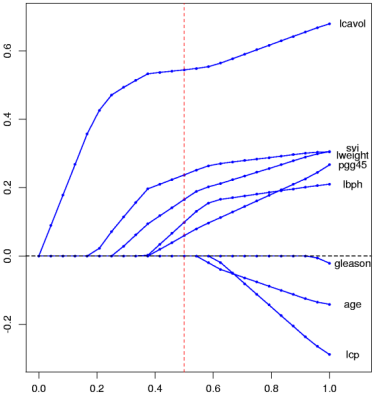
\includegraphics[width=0.6 \linewidth]{chapters/svm/images/L_1.png}
    \label{fig:image}    
\end{align*}

\begin{itemize}
    \item \(L_2\) регуляризатор: \(\mu \sum_{j} w_j^2\)
\end{itemize}

\begin{align*}
    \centering
    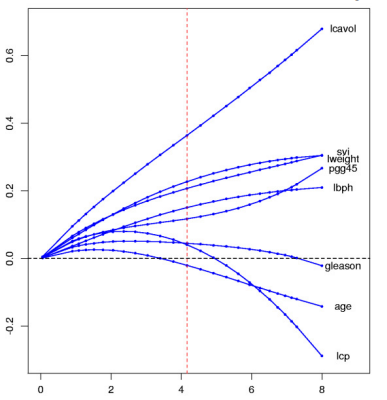
\includegraphics[width=0.6 \linewidth]{chapters/svm/images/L_2.png}
    \label{fig:image}    
\end{align*}

\section{Doubly Regularized SVM (Elastic Net SVM)}

\begin{align*}
    C \sum_{i=1}^{\ell} \left(1 - M_i(w, w_0)\right)_+ + \mu \sum_{j=1}^{n} |w_j| + \frac{1}{2} \sum_{j=1}^{n} w_j^2 & \rightarrow \min_{w, w_0}
\end{align*}

\subsection*{Плюсы:}
\begin{itemize}
    \item Параметр селективности \(\mu\) управляет отбором признаков: чем больше \(\mu\), тем меньше признаков останется
    \item Есть эффект группировки (grouping effect): значимые зависимые признаки отбираются вместе
\end{itemize}

\subsection*{Минусы:}
\begin{itemize}
    \item Шумовые признаки также группируются и могут вместе оставаться в модели
    \item Приходится подбирать два параметра регуляризации \(\mu, \tau\) (есть специальные методы, например, regularization path)
\end{itemize}

\subsection{Elastic Net Analysis}

Elastic Net менее жёстко отбирает признаки.

\begin{figure}[h]
    \centering
    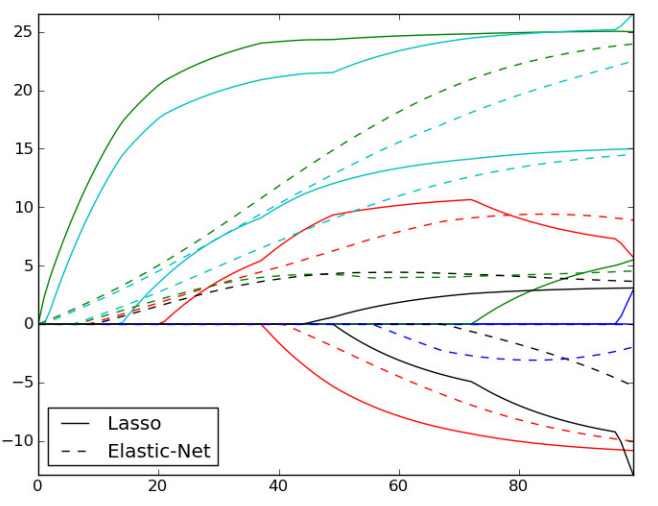
\includegraphics[width=0.8\linewidth]{chapters/svm/images/Elastic_Net.png}
    \caption{Зависимости весов \(w_j\) от коэффициента \(\log \frac{1}{\mu}\)}
    \label{fig:mpr}
\end{figure}

\section{Support Features Machine (SFM)}

\begin{align*}
    C \sum_{i=1}^{\ell} \left(1 - M_i(w, w_0)\right)_+ + \sum_{j=1}^{n} R_{\mu}(w_{j}) & \rightarrow \min_{w, w_0}
\end{align*}

\begin{align*}
R_{\mu}(w_j)=
    \begin{cases}
        2\mu |w_j|, & |w_j| \leq \mu\\
        \mu^2 + w_j^2, & |w_j| \geq \mu \\
    \end{cases}
\end{align*}

\subsection*{Плюсы}
\begin{itemize}
    \item Только один параметр регуляризации \(\mu\)
    \item Отбор признаков с параметром селективности \(\mu\)
    \item Эффект группировки: значимые зависимые признаки ($|w_j|$ > \(\mu\)) входят в решение совместно (как в $Elastic$ $Net$)
    \item Шумовые признаки ($|w_j|$ < \(\mu\)) не группируются и подавляются независимо друг от друга (как в $LASSO$)
\end{itemize}

\section{Relevance Features Machine (RFM)}

\begin{align*}
    C \sum_{i=1}^{\ell} \left(1 - M_i(w, w_0)\right)_+ + \sum_{j=1}^{n} \ln(w_j^2 + \frac{1}{\mu}) & \rightarrow \min_{w, w_0}
\end{align*}

\begin{align*}
    R(w) = \ln(w^2 + \frac{1}{\mu}), \quad \mu = 0.1, 1, 100
\end{align*}

\subsection*{Плюсы}
\begin{itemize}
    \item Только один параметр регуляризации \(\mu\)
    \item Отбор признаков с параметром селективности \(\mu\)
    \item Есть эффект группировки
    \item Лучше отбирает набор значимых признаков, когда они только совместно обеспечивают хорошее решение
\end{itemize}

\section{Задачи}

\subsection{Задача 1}

Качественно объяснить, почему $L_1$-регуляризатор приводит к отбору признаков

\subsection{Ответ:}

Аппроксимация эмпирического риска с \(L_1\)-регуляризацией:
\begin{align*}
    \sum_{i=1}^{\ell} \left(1 - M_i(w, w_0)\right)_+ + \mu \sum_{j=1}^{n} |w_j| & \rightarrow \min_{w, w_0}
\end{align*}

\textcolor{red}{Почему \(L_1\)-регуляризатор приводит к отбору признаков?}

Замена переменных: 
\[
u_j = \frac{1}{2} (|w_j| + w_j), \quad v_j = \frac{1}{2} (|w_j| - w_j).
\]
Тогда 
\[
w_j = u_j - v_j \quad |w_j| = u_j + v_j.
\]

\begin{align*}
    \sum_{i=1}^{\ell} \left(1 - M_i(u - v, w_0)\right)_+ + \mu \sum_{j=1}^{n} (u_j + v_j) & \rightarrow \min_{u, v}, \\
    u_j \geq 0, \quad v_j \geq 0, \quad j = 1, \ldots, n.
\end{align*}

чем больше \(\mu\), тем больше индексов \(j\) таких, что \(u_j = v_j = 0\), но тогда \(w_j = 0\), значит, \textcolor{red}{признак не учитывается.}

\subsection{Задача 2}

Привести пример нежелательного эффекта в процессе обучения, с которым поможет справиться регуляризация 
 
\subsection{Ответ:}

Регуляризация помогает в случае линейной зависимости (мультиколлинеарности) признаков:\\
Пусть построен классификатор: $a(x, w) = sign\langle w, x \rangle$ \\
Мультиколлинеарность: $\exists$  $u \in \mathbb{R}^{n}$: $\forall x \in X$ $\langle u, x \rangle = 0$ \\
Неединственность решения и рост нормы вектора весов: $\forall \gamma \in \mathbb{R}$ $a(x, w) = sign\langle w, x \rangle = sign \langle w + \gamma u, x \rangle$ \\
\\
Проявления переобучения:
\begin{itemize}
    \item слишком большие веса $|w_j|$ разных знаков
    \item неустойчивость дискриминантной функции $\langle w, x \rangle$
    \item $Q(X^{\ell}) \ll Q(X^{k})$
\end{itemize}
Способ уменьшить переобучение:\\
регуляризация $||w|| \rightarrow min$ (сокращение весов, $weight$ $decay$)

\subsection{Задача 3}

Дана задача оптимизации:
\begin{align*}
    \frac{1}{2}(wx - b)^2 + \lambda|w| & \rightarrow \min_{w},
\end{align*}
где $x,$ $b$ $\in \mathbb{R};$ $\lambda \geq 0$\\
При каких $\lambda$ данная задачи имеет решение $w_0 \neq 0?$
 
\subsection{Ответ:}

Находим правую и левую односторонние производные в нуле и рассматриваем, когда они больше и меньше 0 соответственно:

\begin{align*}
    \begin{cases}
        -xb + \lambda > 0\\
        -xb - \lambda < 0\\
        \lambda \geq 0\\
    \end{cases} \Leftrightarrow \lambda > |xb|
\end{align*}

Это условие на $\lambda,$ при котором задача имеет решение $w_0 = 0,$ поэтому нам подходит $\lambda \in [0;$ $|xb|)$.
